\begin{document}
	
	\chapter{Invatare automata}
	
		\begin{center}
		"Orice aspect al invatarii sau caracteristica a inteligentei poate fi descrisa atat de precis incat o masina poate fi facuta sa o simuleze"\cite{mccarthy_proposal} 
		\end{center}
	
	Invatarea este definita ca fiind achizitia cunostiintelor sau a aptitudinilor prin studiu, experienta sau prin invatare. Definitia acopera intr-un mod minimal modalitatea de functionare a invatarii automate in randul sistemelor. Pentru a putea fi cababili de a invata o masina cum sa ia decizii intr-un mod asemanator creierului uman, este necesara intelegerea gandirii umane. Acest lucru poate fi realizat prin introspectie sau prin experimente psihologice.  
	Fundamente de baza ale invatarii automate pot fi regasite de asemenea in comportamentul si abilitatea de invatare a animalelor. Un exemplu concret ar fi modul in care sobolanii reactioneaza la hrana cu miros sau aspect nefamiliar. Acestia vor lua cantitati mici din hrana la inceput, iar bazat pe gust si efectul asupra lor, vor lua progresiv cantitati mai mari. Daca hrana are un efect negativ asupra sobolanilor, nu doar ca nu o vor manca dar vor folosi experienta in viitor cand vor fi pusi din nou in fata unui miros sau aspect nefamiliar, evitand hrana. 
	
	\section{Aspecte generale}
	Abilitatea sistemelor de a lua decizii fara o indrumare explicita a fost o provocare pentru multe domenii stiintifice, iar procesul de descoperire este inca in derulare, avand un progres vizibil in ziua de astazi. La baza acestei capabilitati ale sistemelor, se afla algoritmi construiti si optimizati pe parcusul istoriei, sustinuti de avansarea tehnologiei si cresterea semnificativa a masei de informatie si a valabilitatii ei. 
	Algoritmii au urmarit mai multe tipologii, care astazi se rezuma la doi: invatare supervizata si invatare nesupervizata. Desi algoritmii invatarii automata difera de la unul la celalalt, scopul lor este comun.
	
	\subsection{Puncte cheie in istoria intelgentei artificiale}
	In prima jumatate a secolului 20 filmele science fiction au adus in lumina inteligenta artificiala prin intermediul a mai multor personaje. Printre primele personaje care sustineau acest concept a fost Tin, omul de tinichea, din vrajitorul din Oz, care a fost urmat la scurt timp de robotul cu caracter uman, Maria, din “Metropolis”. Prezenta acestor personaje scoate in evidenta interesul, chiar daca involuntar, a oamenilor in abilitatea unor sisteme de a prelua comportamentul celui mai complex lucru din lume pana in momentul de fata, creierul uman. 
	
	Pana in anii 50 lumea s-a bucurat de o generatie de cercetatori in stiinta, matematica si filozofie care aveau un tel comun, si anume, aducerea din filme si fictiune a “sistemelor inteligente” la realitate. Printre acele persoane se enumara si Alan Turing, o personalitate remarcabila in IT-ul de astazi de care lumea se bucura si profita. Turing a folosit o interpretare matematica pentru a demonstra posibilitatea de existenta a inteligentei masinariilor,un domeniu nedefinit la momentul acela. Acesta era de parere ca daca oamenii pot rezolva o problema utilizand un motiv si informatii, un calculator ar putea sa faca la fel. \cite{ai_history}
	
	In 1950, Alan Turing vine cu o lucrare care va avea sa incepea cu fraza “Can machines think?”. Lucrarea va avea sa puna bazele metodelor prin care masinile inteligente sunt construite si testate. Acesta face o analogie, in lucrarea sa, intre inteligenta artificiala si un joc pe care acesta il numeste “The Imitation Game”, care este alcatuit din 3 jucatori: Un barbat, reprezentat prin A, o femeie, reprezentata prin B, si un interogator. Interogatorul sta intr-o alta camera decat barbatul si femeia. Scopul interogatorului este sa isi dea seama, pana la finalul jocului, care dintre A si B este femeia si care este barbatul. Acesta poate pune intrebari fiecaruia, in scopul de a-si da seama din descriere genul persoanei intrebate. Intrebarea va fi pusa atunci cand un calculator va lua locul lui A sau B. Va creste nivelul dificultatii pentru interogator ? Alan Turing si-a sustinut intrebarea de la inceputul  articolului prin aceasta analogie. \cite{turing}
	
	In 1955, avea sa fie conturat acest domeniu, al masinilor inteligente, pentru prima data, de catre omul de stiinta John McCarthy, recunoscut in zilele de astazi, ca si fiind tatal inteligentei artificiale. Acesta a inventat si a definit domeniul inteligentei artificiale, prin propunerea sa de lucrarea, la conferinta ce a avut loc in anul 1956 la Dartmouth. Lucrarea sa urmarea sa exploreze posibilitatile de intelegere, invatare si auto-dezvoltare a unei masini. Acesta considera ca orice act de inteligenta a omului este studiat si  inteles la un nivel atat de ridicat,  incat ar putea fi transpus in rutina calculatoarelor. Anul 1958, John McCarthy creeaza limbajul de programare LISP, care va deveni limbajul de baza a inteligentei artificiale si va avea sa ramana astfel pana in zilele de astazi. [5]
	John McCarthy a pus bazele unui domeniu care este studiat intensiv si in momentul actual si care nu are un progres liniar si predictiv. Acesta considera, la acel moment, ca apogeul inteligentei artificiale ar putea aparea in 5 ani, sau ar putea aparea in 500 de ani, dar nu a negat niciodata posibilitatea de dezvoltare si avansare a acestui domeniu.
	
	
	\subsection{Cum functioneaza?}
	Invatarea automata urmareste un sablon, a carui scop este dezvoltarea unui model capabil de a separa datele de intrare, in grupuri care au aspecte comune, astfel putand sa le clasifice. Datele de intrare sunt adesea distribuite in asa fel incat trasarea unei linii drepte in plan nu va putea clasifica corect datele, astfel  modelul va trebui sa gaseasca o corelatie neliniara intre datele care ii sunt date si rezultatul care va servi ca predictie a sa. (Vezi Figura \ref{fig:uml-diagram})
	

	
	\begin{figure}[H]
		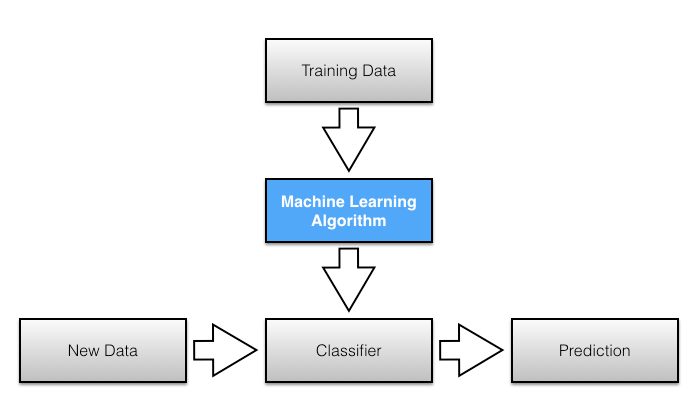
\includegraphics[width=15cm]{ml-uml}  
		\caption{\label{fig:uml-diagram} Diagrama generala a algoritmului de invatare supervizata
		\protect
		\cite{ml_intro}}
	\end{figure}


	\newpage
	
	Modul de functionare al algoritmilor de invatare automata este dat de clasificarea lor in cele doua tipuri, invatare supervizata si invatare nesupervizata. Punctul cheie care face diferenta intre aceste doua tipuri de algoritmi, este aprovizionarea invatarii cu clase de clasificare si date de validare, in cazul invatarii supervizate. Algoritmul invatarii nesupervizate este bazat pe un curs “instinctiv” i.e. modalitate de clasificare si impartire este lasata la latitudinea masinii.
	
	Invatarea automata supervizata este bazata pe perechi alcatuite din date de intrare si o “eticheta” atribuita fiecarei date de intrare. Algoritmul va modela o functie, bazata pe aceste perechi de intrare, iar scopul final este de a atribui corect unei valori arbitrare, nefamiliare algoritmului, o eticheta corespunzatoare din cele care i-au fost aprovizionate in etapa de invatare. 
	In contrast, invatarea automata nesupervizata este bazata doar pe date de intrare, astfel algoritmul fiind obligat sa gestioneze informatia fara a fi indrumat. Avantajul acestui algoritm este faptul ca poate gestiona probleme complexe, superioare creierului uman, prin faptul ca va crea sau va atribui clase unor grupuri de date de intrare, bazat pe similaritati descoperite pe parcurs.
	Alegerea tipului de invatare va fi data de complexitatea si structura  datelor de intrare cat si de scopul problemei. Nu este exclusa posibilitatea utilizarii celor doua metode concomitent, adeseori ducand la rezultate mai concise.
	
	\subsection{Aplicabilitate}
	Invatarea automata se regaseste in multe activitati ale societatii moderne, se extinde pe diferite planuri si acopera nevoi de zi cu zi ale oamenilor. De la sugestii pe site-uri de muzica si clipuri video, filtrarea reclamelor si a continutului de pe site-uri de socializare  si pana la masini cu functionalitate de parcare automata, invatarea automata este raspunsul problemelor de gestionare si clasificare a evenimentelor si a stimulilor externi. 
	Invatare automata se intinde pe diferite domenii acoperind nevoi de baza dar exceland si in aplicatii mai complexe.
	
	Printre domenii in care inteligenta artificiala si invatarea automata si-au lasat amprenta, se enumera:
	
	\begin{itemize}
		\item Masini inteligente. Invatarea automata, impreuna cu senzorii de pe masini, au adus o multitudine de functionalitati utile. Astazi masinile se pot parca si conduce singure si pot evita un accident iminent.
		
		\item Securitatea datelor. Virusii de tip Malware sunt o problema persistenta din punctul de vedere al datelor personale ce prezinta o valoare pentru un atacator. Invatarea automata ajuta in combatarea acestei probleme prin depistarea fisierelor noi aparute de malware.
		
		\item Tranzactii financiare. Invatarea automata este folosita de multi giganti ai pietei de capital si bursa, pentru realizarea unor schimburi automatizate cat mai precise
		
		\item Sanatate. Algoritmii predictivi sunt astazi un factor important in detectarea precoce a unor probleme de sanatate, cum ar fi cancerul.
		
		\item Detectarea de fraude bancare. Bazat pe invatarea automata, bancile pot detecta cand are loc o tranzactie fraudulenta sau spalare de bani, bazat pe detaliile acelei tranzactii.			
	\end{itemize}
	
	\vfill
	
	
	\section{Procesarea de imagini}
	Domeniul procesarii de imagini nu poate fi definit sau clasificat printr-o simpla categorie. Acesta a fost si este intr-o continua dezvoltare si urmareste mai multe planuri. 
	
	Importanta acestor imagini digitale, se poate resimti pe multe domenii. Bazat pe aceste reprezentari si pe abilitati dobandite pana in prezent in materie de procesare si prelucrare, am obtinut diferite rezultate si aplicabilitati
	
	\subsection{Problema procesarii imaginilor}
	Problema procesarii imaginilor se rezuma la procesul de invatare a unui sistem cu abilitati pseudo-cognitive de a lua decizii pe baza unor detalii sau a unor caracteristici ale imaginii. Sistemul poate fi invatat, prin intermediul algoritmilor, sa extraga caracteristici spre a le refolosi, sau poate utiliza date deja existente in scopul gasirii unor similaritati. 
	
	Exista diferite reprezentari ale imaginilor pe sisteme, definite ca si fiind formaturi. Unitatea de baza a imaginii este pixel-ul. Pixel este o prescurtare provenita de la Picture Element, si reprezinta un punct de la o pozitie x, y a ecranului. In functie de format, pixelul reprezinta proprietati ale elementului de pe pozitia x, y; astfel de proprietati pot fi culoarea si optional, opacitatea elementului.O multitudine de pixel, fiecare cu proprietatiile proprii, reprezinta reprezentarea unei imagini. \cite{image_representation}
	
	\subsection{O noua perspectiva. Retele Neuronale}
	Studiul creierului uman si a modului sau de functionare a deschis porti noi in domeniul stiintei. Felul in care neuronii cumunica prin sinapse si isi intaresc legaturile cele mai des folosite, a inspirat oameni de stiinta in creare unei analogii in domeniul stiintific, care va avea sa rezolve probleme asemanatoare celor pe care creierul le gestioneaza.
	
	In 1943, idea unei  lucrari care prezenta modul de functionare a creierului, semnata de  neurofiziologul Warren McClulloch si matematicianul Walter Pitts,   a fost sustinuta practic prin simularea functiilor neuronilor si a legaturile dintre ei, prin circuite electrice. Retelele neuronale fizice, reprezentate prin circuite electrice, au fost primul stimulent care a introdus o noua perspectiva in rezolvarea problemelor inca din inaintea dezvoltarii domeniului inteligentei artificiale. 
	
	
	Retelele neuronale artificiale au ca unitate de baza neuronul artificial, care primeste unul sau mai multe semnale de intrare (asociate cu potentialul postsinaptic excitator si potentialul postsinaptic inhibator), care insumate vor rezulta un semnal de iesire. Acest semnal de iesire este mai apoi trecut printr-o functie de activare (functie de transfer) pentru a combate rezultatul linear al insumarii semnalelor de intrare ale neuronului. (Vezi Fig. \ref{fig:neuron-schema})
	
	\begin{figure}[H]
		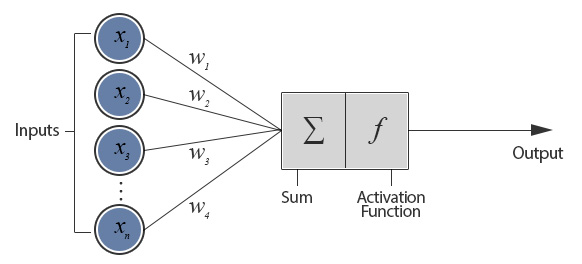
\includegraphics[width=15cm]{neuron-schema}  
		\caption{\label{fig:neuron-schema} Diagrama neuron artificial 
		\protect 
		\cite{ann}}
	\end{figure}
	
	
	Un model predictiv de retele neuronale este alcatuit din mai multe straturi de neuroni, lucrand impreuna pentru o modela o functie non-lineara complexa.
	Fiecare strat va avea propriile proprietati, cum ar fi: numarul de neuroni, ponderile aferente si functia de activare.
	
	Procesul in care date sunt procesate, prin straturile de neuroni intermediare, se numeste operatie feed-forward. La finalul operatiei feed-forward, algoritmul va prezenta datele asupra carora s-a aplicat o mutatie. Pe baza acestor date, algoritmul va verifica rezultatul obtinut comparandu-l cu un set de date de antrenare. 
	
	Odata ce eroare a fost obtinuta, aceasta va circula in sens invers prin straturile de neuroni si va ajusta ponderile ce au influentat decizia luata de model.
	
	

\end{document}